\section{实验设计}

\subsection{控制器(Controller)}\label{sub:controller}

\subsubsection{功能描述}
由maindec和aludec两部分组成,通过输入32位指令的operation code和function code,得到各多选器,ALU,存储器的控制信号
\newpage
\subsubsection{接口定义}

\begin{table}[htp]
\caption{接口定义}\label{tab:signaldef}
\begin{center}
	\begin{tabular}{lllp{6cm}}
	\hline
	\textbf{信号名} & \textbf{方向} & \textbf{位宽} & \textbf{功能描述}\\ \hline
	op		& Input & 6-bit & 32位指令的高六位 operation code\\ 
	func	& Input & 6-bit & 32位指令的低六位 function  code\\
	jump    & Output& 1-bit & 如果是无条件跳转指令为1,否则为0\\
	branch  & Output& 1-bit & 如果是条件跳转指令为1,否则为0 \\
	alusrc  & Output& 1-bit & 如果alu的第二个操作数来自于低16位符号拓展为1,否则为0\\
	memwrite& Output& 1-bit & 数据存储器写使能有效为1,否则为0\\
	memtoreg& Output& 1-bit & 写入寄存器的数据来自数据存储器为1,否则为0\\
	regwrite& Output& 1-bit & 寄存器堆写使能有效为1,否则为0\\
	regdst  & Output& 1-bit & 写寄存器的目标寄存器号来自rd字段为1,来自rt字段为0\\
	pcsrc   & Output& 1-bit & pc由分支地址取代为1,pc+4为0\\
	alucontrol&Output&3-bit & ALU控制信号,由funct(5:0)和op(31:26)共同决定\\
	\hline
	\end{tabular}
\end{center}
\end{table}

\subsubsection{逻辑控制}
\begin{enumerate}
\item 采用组合逻辑设计控制器,其中aludec采用assign赋值语句,maindec采用always赋值
\item 根据不同指令的功能分析其所需要的路径,分析数据通路图,判断指令是否需要写寄存器、访存等等操作,以产生相应的控制信号,即可得到信号所对应的值。
\end{enumerate}

\subsection{存储器(Block Memory)}\label{sub:ctl}

\subsubsection{类型选择}
根据实验指导书内容,调用Block Memory Generator
\begin{enumerate}
    \item Flow Navigator->IP Catalog,在搜索栏直接搜索 Block Memory Generator
    \item Interface Type : Native
    \item Generate address interface with 32bits : 未选
    \item Memory Type : Single Port RAM
    \item Write\_Read Width : 32
    \item Write\_Read Depth : 1024
    \item Operating Mode : Read First
    \item Enable Port Type : Always Enabled
    \item Primitives Output Register : 选中
    \item Fill Remaining Memory Locations : 选中
\end{enumerate}

\subsubsection{参数设置}

\begin{figure}[htbp]
    \centering
    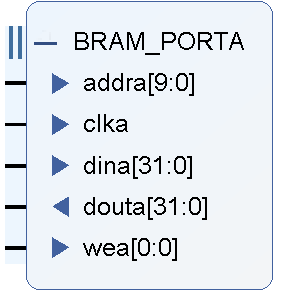
\includegraphics[width=0.2\textwidth]{ip.png}
    \caption{BMG ip核}
    % \label{fig:my_label}
\end{figure}

\begin{enumerate}
    \item addra : 10位指令存储器地址
    \item clka  : 时钟信号
    \item dina  : 32位写输入
    \item douta : 32位读输出
    \item wea   : 0位写使能信号
\end{enumerate}
